% !TEX TS-program = xelatex
\documentclass{article}

\usepackage[T1]{fontenc}
\usepackage[utf8]{inputenc}

\usepackage{graphicx}
\graphicspath{{assets/}}

\usepackage{polyglossia}
\usepackage{hyperref}

\hypersetup
{
  pdftitle   = {Computer Vision – Assignment 2},
  pdfauthor  = {Markus Reiter}
}

\title{Computer Vision – Assignment 2}
\author{Markus Reiter}

\begin{document}

\maketitle

  \section{Spatiotemporal Filtering}

  The purpose of this assignment was to extract motion from a video, that is, separating the static parts of a video from the ones containing motion. The hypothesis here is that we can detect motion by comparing the pixels of multiple frames of a video. If pixels with the same brightness stay at the same position, there is no motion, if they move to a different position, there is. To make this difference visible, we can interpolate over multiple frames. This is exactly the purpose of a spatiotemporal filter. It is applied on one axis, either x or y, and the time-axis which in case of videos consists of frames.

  Our solution was implemented in Matlab. We used \texttt{VideoReader} to read the video file as a matrix, after which we converted every frame to grayscale using \texttt{rgb2gray}. All frames were then concatenated to a \texttt{frames} vector.

  The second part was the function \texttt{energyOfGabor(video, gabor\_size, sigma, theta)}. In this function, a Gabor filter is generated using the function given in the assignment and using the variables passed to \texttt{energyOfGabor}. The \texttt{video} variable corresponds to the \texttt{frames} variable, which is ordered like this: \texttt{[height, width, frame]}. We then use \texttt{size(video, 2)} to get the width, in order to be able to loop through the x-axis. In each iteration of this loop, we then have a matrix of \texttt{[height, frame]} pixels, i.e. a column of the video. We get this column using \texttt{squeeze(video(:, col, :))}, and convolve it once using \texttt{g\_even}, and once using \texttt{g\_odd} with the \texttt{conv2} function. We then take the sum of the square of both of these, and then take the square root. We append the resulting column to an array. This array will have the form \texttt{[height, frame, width]}, so we have to permutate it once using the \texttt{permutate} function in order to look like the input array: \texttt{[height, width, frame]}.

  For the Nine-Tap filter, we use the same approach as for the \texttt{energyOfGabor} function. Inside the loop, we convolve one with our filter \texttt{f1}, and once with the filter \texttt{f2}. We then do an element-wise multiplication of the two resulting columns and append them to the output array.

  In our main program, either \texttt{energyOfGabor} or \texttt{nineTap} is called and its result is displayed with \texttt{implay}.

  \subsection{Results}

  With the Gabor filter, there is a clear distinction between moving and still parts of a video. In our case, we used a Gabor filter of size 9, which gave the best result. The Nine-Tap filter does have a lot of noise, which is presumably because it is only a filter of size 3, but even though there is a lot of noise, the motion can be clearly distinguished from the noise.

  \begin{figure}[!ht]
    \caption{Energy of Gabor}
    \centering
    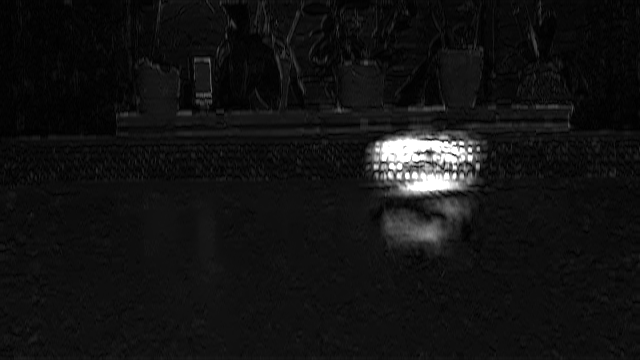
\includegraphics[width=.8\textwidth]{gabor.png}
  \end{figure}

  \begin{figure}[!ht]
    \caption{Nine-Tap Filter}
    \centering
    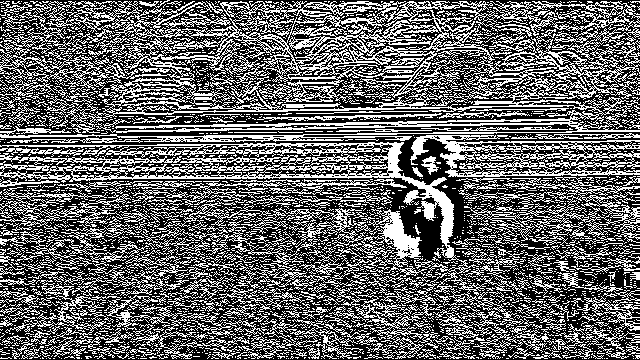
\includegraphics[width=.8\textwidth]{nine-tap.png}
  \end{figure}

\end{document}
